187. \begin{figure}[ht!]
\center{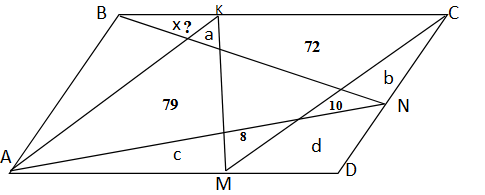
\includegraphics[scale=0.6]{g8-187.png}}
\end{figure}\\
Так как формула нахождения площади треугольника отличается от формулы нахождения площади параллелограмма только множителем $\cfrac{1}{2},$ имеем равенства
$\cfrac{1}{2}S_{ABCD}=S_{\Delta BNC}+S_{\Delta AND}=S_{\Delta AKM}+S_{\Delta CMD},$ откуда $x+a+72+b+c+8+d=a+79+c+b+10+d,\ x=9.$\\
